\subsection{Uneven movement}
The DBRS algorithms assumes, that the target moves like straight paths and does not change direction to go backwards. The bad scenarios is sketched in figure-\ref{unevenmovement}.

\begin{figure}
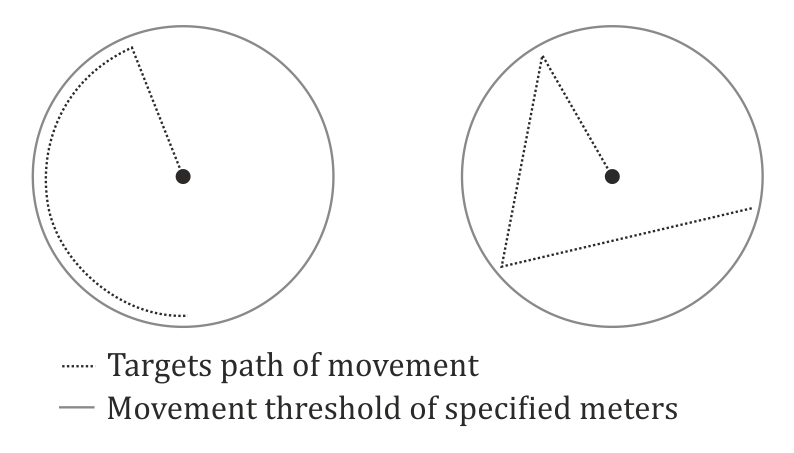
\includegraphics{UnevenMovement}
\label{unevenmovement}
\caption{Examples of how some kinds of movement can give trouble with the distance based algorithms}
\end{figure}

The left circle shows a target, which moves to the circumference of the movement threshold and then follow the circumference at the inside. It results in no location is sent to the server, due to the threshold is never crossed, and a lot of GPS fixes, due to the small distance to the circumference.

The right circle shows a situation, where the target moves in one direction and then change direction to backwards. If the target only moves around inside the threshold circle the server will not get any location updates.

These conditions has to be evaluated according to the use case, where it can be determined whether these scenarios will occur. In the case where a person walks or a car drives towards some locations it is unlikely, that these scenarios will occur.